% Drawing 148/04-5 -- folder 148, batch 04, archive page 68 (PDF page 69).
% Transcription: un seul dessin, sans texte : une carte triangulée au crayon, dont les seize sommets sont entourés de petits cercles à l'encre rouge marqués $0$, $1$ ou $\infty$, dix demi-droites partant des sommets du pourtour ; autour d'un sommet central, une famille de courbes fermées emboîtées à l'encre rouge, qui englobent les sommets de proche en proche --- un découpage en « pantalons ».
% Kind: triangulated map with ringed vertices and nested red curves (pants decomposition). Method 2 (schematic redraw from the facsimile). Status: partial.
% Notes: Colour render; same kind of figure as 04-2 (p. 71). Drawn: the sixteen vertices at their places, each with its red ring; the pencil edges read on the crop (twenty-three), every edge between its two vertex points; the ten half-lines going off from the outer vertices; in red, nine nested closed curves around the central pair of vertices. Left out: the labels 0, 1, infinity written in the rings (too small to read reliably on the render; the edges read are compatible with neighbours carrying different labels), and the small arrow ticks on the red curves. Still differs, and this is the main defect: the red curves are an interpolated family between the innermost and the outermost curve of the page, so the redraw shows the nesting but not which vertices each curve encloses, nor the places where the curves pinch around a ring; some faint pencil edges may be missing or wrongly joined. The figure is not encoded for the same reason. Redrawn 2026-11-12 (issue 128): to check again.
% Coordinates: 1 unit = 1 mm = 1/100 of the crop width, y downwards as on the crop (bbox in page fractions: [0.18, 0.075, 0.8, 0.36]).
% Redrawn by Claude (claude-fable-5-2), issue #128, 2026-11-12; not checked by a human; not compiled (no TeX in the session).
% Rights: reproduces part of the work -- behind RENDER_TRANSCRIPTS, never published by itself.
\documentclass[tikz,border=3pt]{standalone}
\usepackage{amsmath,amssymb}
\usetikzlibrary{patterns,arrows.meta}
\tikzset{pencil/.style={black!45}, struck/.style={black!35}, mpt/.style={circle,draw,inner sep=1.3pt}, pt/.style={circle,fill,inner sep=0.9pt}, opt/.style={circle,draw,fill=white,inner sep=1.1pt}, Rd/.style={red!75!black}, Gn/.style={green!45!black}, Br/.style={brown!70!black}}
\begin{document}
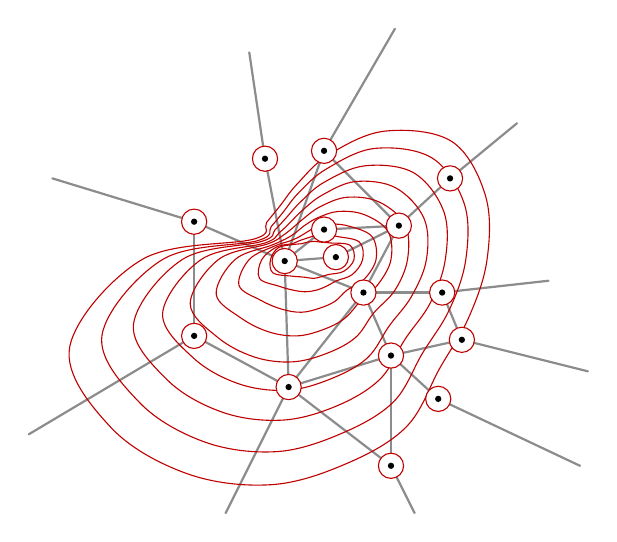
\begin{tikzpicture}[x=1mm,y=-1mm,line cap=round,line join=round,font=\small]
\coordinate (a) at (40,20);
\coordinate (b) at (47.5,19);
\coordinate (c) at (63.5,22.5);
\coordinate (d) at (31,28);
\coordinate (e) at (47.5,29);
\coordinate (g) at (57,28.5);
\coordinate (o) at (42.5,33);
\coordinate (h) at (49,32.5);
\coordinate (i) at (52.5,37);
\coordinate (j) at (62.5,37);
\coordinate (k) at (31,42.5);
\coordinate (l) at (65,43);
\coordinate (m) at (56,45);
\coordinate (n) at (43,49);
\coordinate (p) at (62,50.5);
\coordinate (q) at (56,59);
\draw[pencil,thick] (o) -- (a);
\draw[pencil,thick] (o) -- (b);
\draw[pencil,thick] (o) -- (e);
\draw[pencil,thick] (o) -- (h);
\draw[pencil,thick] (o) -- (i);
\draw[pencil,thick] (o) -- (d);
\draw[pencil,thick] (o) -- (n);
\draw[pencil,thick] (e) -- (g);
\draw[pencil,thick] (h) -- (g);
\draw[pencil,thick] (g) -- (c);
\draw[pencil,thick] (g) -- (i);
\draw[pencil,thick] (i) -- (j);
\draw[pencil,thick] (j) -- (l);
\draw[pencil,thick] (i) -- (m);
\draw[pencil,thick] (m) -- (l);
\draw[pencil,thick] (m) -- (n);
\draw[pencil,thick] (n) -- (i);
\draw[pencil,thick] (n) -- (k);
\draw[pencil,thick] (k) -- (d);
\draw[pencil,thick] (n) -- (q);
\draw[pencil,thick] (m) -- (q);
\draw[pencil,thick] (p) -- (m);
\draw[pencil,thick] (b) -- (g);
\draw[pencil,thick] (a) -- (38,6.5);
\draw[pencil,thick] (b) -- (56.5,3.5);
\draw[pencil,thick] (c) -- (72,15.5);
\draw[pencil,thick] (j) -- (76,35.5);
\draw[pencil,thick] (l) -- (81,47);
\draw[pencil,thick] (p) -- (80,59);
\draw[pencil,thick] (q) -- (59,65);
\draw[pencil,thick] (n) -- (35,65);
\draw[pencil,thick] (k) -- (10,55);
\draw[pencil,thick] (d) -- (13,22.5);
\draw[Rd] plot[smooth cycle,tension=0.6] coordinates {(51.3,32.8) (50,34.3) (48.1,34.7) (47.1,35) (46.2,35.2) (45.4,35.1) (44.5,35) (43.3,34.9) (41,34.5) (40.7,32.8) (41.7,31.3) (43.6,30.9) (44.6,30.8) (45.4,30.6) (46.2,30.5) (47.1,30.6) (48.3,30.7) (50.8,31)};
\draw[Rd] plot[smooth cycle,tension=0.6] coordinates {(52.4,32.8) (51.1,34.7) (49.1,35.5) (47.8,36.2) (46.5,36.7) (45.1,36.9) (43.6,36.7) (41.8,36.2) (39.3,35.2) (39.6,32.8) (41.5,31.2) (43.4,30.8) (44.4,30.4) (45.3,30.1) (46.3,29.8) (47.6,29.7) (49.3,29.9) (52,30.6)};
\draw[Rd] plot[smooth cycle,tension=0.6] coordinates {(54.1,32.8) (52.6,35.3) (50.4,36.7) (48.9,38.1) (46.9,39) (44.6,39.5) (42.1,39.1) (39.5,38) (36.7,36.1) (38,32.8) (41.2,31.1) (43,30.5) (44.2,30) (45.2,29.4) (46.5,28.7) (48.4,28.3) (50.8,28.6) (53.6,29.9)};
\draw[Rd] plot[smooth cycle,tension=0.6] coordinates {(56,32.8) (54.4,35.9) (52.1,38.1) (50.1,40.3) (47.4,41.7) (44.1,42.5) (40.5,42) (36.9,40.2) (33.8,37.2) (36.2,32.8) (40.8,31) (42.6,30.2) (43.9,29.4) (45,28.5) (46.7,27.5) (49.3,26.7) (52.6,27.1) (55.6,29.2)};
\draw[Rd] plot[smooth cycle,tension=0.6] coordinates {(58.1,32.8) (56.5,36.7) (53.8,39.6) (51.5,42.7) (47.9,44.7) (43.5,45.8) (38.7,45.2) (34,42.7) (30.5,38.4) (34.1,32.8) (40.4,30.8) (42.2,29.8) (43.5,28.8) (44.9,27.6) (47,26.1) (50.4,24.9) (54.5,25.5) (57.8,28.4)};
\draw[Rd] plot[smooth cycle,tension=0.6] coordinates {(60.5,32.8) (58.6,37.5) (55.8,41.2) (53,45.3) (48.5,47.9) (42.9,49.4) (36.7,48.6) (30.9,45.3) (27,39.6) (31.9,32.8) (40,30.7) (41.8,29.4) (43.1,28.2) (44.7,26.6) (47.3,24.6) (51.5,22.9) (56.6,23.7) (60.2,27.6)};
\draw[Rd] plot[smooth cycle,tension=0.6] coordinates {(62.9,32.8) (61,38.3) (57.8,42.9) (54.6,48) (49.1,51.4) (42.2,53.2) (34.6,52.2) (27.6,48.1) (23.3,41) (29.5,32.8) (39.6,30.5) (41.3,29) (42.7,27.5) (44.5,25.5) (47.5,23) (52.7,20.9) (58.9,21.8) (62.7,26.7)};
\draw[Rd] plot[smooth cycle,tension=0.6] coordinates {(65.5,32.8) (63.4,39.2) (60,44.7) (56.3,50.9) (49.7,54.9) (41.5,57.2) (32.4,56) (24.1,51) (19.3,42.4) (27,32.8) (39.1,30.4) (40.8,28.6) (42.3,26.8) (44.3,24.3) (47.8,21.3) (53.9,18.7) (61.2,19.9) (65.3,25.7)};
\draw[Rd] plot[smooth cycle,tension=0.6] coordinates {(68.2,32.8) (65.9,40.1) (62.2,46.6) (58,54) (50.4,58.7) (40.8,61.4) (30.1,60) (20.4,54.1) (15.2,43.9) (24.4,32.8) (38.6,30.2) (40.2,28.1) (41.9,26) (44.1,23.2) (48.1,19.5) (55.2,16.5) (63.7,17.8) (68,24.7)};
\draw[Rd,fill=white] (a) circle [radius=1.6];
\draw[Rd,fill=white] (b) circle [radius=1.6];
\draw[Rd,fill=white] (c) circle [radius=1.6];
\draw[Rd,fill=white] (d) circle [radius=1.6];
\draw[Rd,fill=white] (e) circle [radius=1.6];
\draw[Rd,fill=white] (g) circle [radius=1.6];
\draw[Rd,fill=white] (o) circle [radius=1.6];
\draw[Rd,fill=white] (h) circle [radius=1.6];
\draw[Rd,fill=white] (i) circle [radius=1.6];
\draw[Rd,fill=white] (j) circle [radius=1.6];
\draw[Rd,fill=white] (k) circle [radius=1.6];
\draw[Rd,fill=white] (l) circle [radius=1.6];
\draw[Rd,fill=white] (m) circle [radius=1.6];
\draw[Rd,fill=white] (n) circle [radius=1.6];
\draw[Rd,fill=white] (p) circle [radius=1.6];
\draw[Rd,fill=white] (q) circle [radius=1.6];
\fill (a) circle [radius=0.4];
\fill (b) circle [radius=0.4];
\fill (c) circle [radius=0.4];
\fill (d) circle [radius=0.4];
\fill (e) circle [radius=0.4];
\fill (g) circle [radius=0.4];
\fill (o) circle [radius=0.4];
\fill (h) circle [radius=0.4];
\fill (i) circle [radius=0.4];
\fill (j) circle [radius=0.4];
\fill (k) circle [radius=0.4];
\fill (l) circle [radius=0.4];
\fill (m) circle [radius=0.4];
\fill (n) circle [radius=0.4];
\fill (p) circle [radius=0.4];
\fill (q) circle [radius=0.4];
\end{tikzpicture}
\end{document}
